\documentclass[12pt,a4paper,twocolumn]{article}
\usepackage[latin1]{inputenc}
\usepackage{amsmath}
\usepackage{amsthm}
\usepackage{amsfonts}
\usepackage{amssymb}
\usepackage{graphicx}
\usepackage{cite}
\usepackage{tikz}
\usetikzlibrary{arrows,shapes,automata,petri}
\usepackage[left=2cm,right=2cm,top=2cm,bottom=2cm]{geometry}

\newtheorem{myDef}{Definition}

\author{Josiah Hanna, David Tamez, and Xiaorong Zhu}
\title{Evolving Petri Networks for High Level Robot Control}
\begin{document}

\maketitle

\begin{abstract}

Petri networks are mathematical models for representing processes. One application of Petri networks is modelling high level robot control. In previous work, this has involved hand coding the Petri networks using the designers knowledge of the target domain. In this paper we show how to use an evolutionary algorithm to automatically generate a correct Petri network for a specific task. 

\end{abstract}

\section{Introduction}

\section{Background}

\subsection{Petri Networks}
Petri networks are mathematical models for representing processes. Formally we define Petri nets as:
\begin{myDef}
A Petri Net is defined as a tuple $(P,T,F,M,W)$ where $P$ is a set of place nodes, $T$ is a set of transition nodes, $F$ is a set of arcs in either $P \times T$ or $T \times P$, $M: P \rightarrow Z$ is an initial marking, and $W: F \rightarrow Z$ is an arc weight function.
\end{myDef}
\begin{figure}[h]
\centering
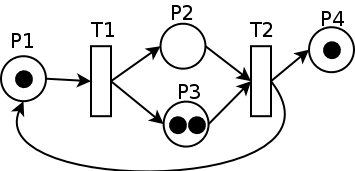
\includegraphics[scale=0.25]{petri_net.png}
\caption[]{An example Petri network \label{exampleNet}}
\end{figure}
Petri nets have many applications including data analysis, simulation of systems, and showing correctness of a system. The techniques we present are for the application of high level robot control. The disadvantage of Petri nets for this application is that they must be hand coded using designer knowledge of the domain. For complex tasks this is not very scalable.

\subsection{The NEAT Algorithm}

\section{Related Work}

\section{Approach}


We propose that the Neuroevolution of Augmenting Topologies (NEAT) could be used to evolve Petri Nets.
\begin{itemize}
\item NEAT evolves topologies and weights of neural networks.
\item NEAT allows complex structures to evolve through speciation.
\item We modify the NEAT genome and mutation operators
\end{itemize}
NEAT becomes PetriNEAT!

Node Genes
\begin{table}
\centering
\begin{tabular}{|c|}
\hline
Node Gene\\ \hline
I.D. \\
Type \\
Initial Tokens \\
Action I.D. \\
\hline
\end{tabular}
\end{table}

Link Gene
\begin{table}
\centering
\begin{tabular}{|c|}
\hline
Arc Gene\\ \hline
Node Place \\
Node Transition \\
Weight \\
\hline
\end{tabular}
\end{table}

We use the following mutation operators in evolving our network:
\begin{itemize}
\item mutate add node
\item mutate add link
\item mutate node
\item mutate link
\end{itemize}

  \begin{figure}
    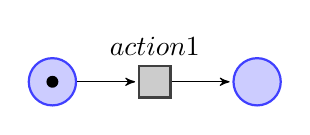
\begin{tikzpicture}[node distance=1.3cm,>=stealth',bend angle=45,auto]
  \tikzstyle{place}=[circle,thick,draw=blue!75,fill=blue!20,minimum size=6mm]
  \tikzstyle{transition}=[rectangle,thick,draw=black!75,
              fill=black!20,minimum size=4mm]
    \node [place,tokens=1] (p1){};
    \node [transition] (t1) [right of=p1, label=above:$action1$] {}  edge [pre] (p1);
    \node [place] (p2)  [right of=t1] {} edge [pre] (t1);
\end{tikzpicture}
\caption{Adding connectivity}
\end{figure}

\begin{figure}
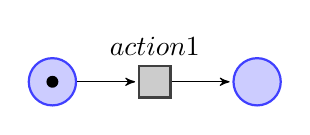
\begin{tikzpicture}[node distance=1.3cm,>=stealth',bend angle=45,auto]
  \tikzstyle{place}=[circle,thick,draw=blue!75,fill=blue!20,minimum size=6mm]
  \tikzstyle{transition}=[rectangle,thick,draw=black!75,
              fill=black!20,minimum size=4mm]
    \node [place,tokens=1] (p1){};
    \node [transition] (t1) [right of=p1, label=above:$action1$] {}  edge [pre] (p1);
    \node [place] (p2)  [right of=t1] {} edge [pre] (t1);
\end{tikzpicture}
\caption{Grow the network}
\end{figure}

  \begin{figure}
    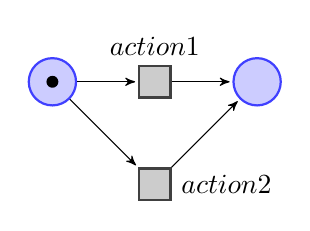
\begin{tikzpicture}[node distance=1.3cm,>=stealth',bend angle=45,auto]
  \tikzstyle{place}=[circle,thick,draw=blue!75,fill=blue!20,minimum size=6mm]
  \tikzstyle{transition}=[rectangle,thick,draw=black!75,
        fill=black!20,minimum size=4mm]
    \node [place,tokens=1] (p1){};
    \node [transition] (t1) [right of=p1, label=above:$action1$] {}  edge [pre] (p1);
    \node [place] (p2)  [right of=t1] {} edge [pre] (t1);
    \node [transition] (p3) [below of=t1, label=right:$action2$] {} edge [pre] (p1) edge [post] (p2);
\end{tikzpicture}
\end{figure}

 \begin{figure}
    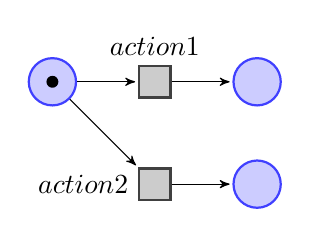
\begin{tikzpicture}[node distance=1.3cm,>=stealth',bend angle=45,auto]
  \tikzstyle{place}=[circle,thick,draw=blue!75,fill=blue!20,minimum size=6mm]
  \tikzstyle{transition}=[rectangle,thick,draw=black!75,
        fill=black!20,minimum size=4mm]
    \node [place,tokens=1] (p1){};
    \node [transition] (t1) [right of=p1, label=above:$action1$] {}  edge [pre] (p1);
    \node [place] (p2)  [right of=t1] {} edge [pre] (t1);
	\node [place] (p4) [below of=p2] {};    
    \node [transition] (p3) [below of=t1, label=left:$action2$] {} edge [pre] (p1) edge [post] (p4);
    
\end{tikzpicture}
\end{figure}


\section{Experiments}

We evolve Petri net solutions for a robot moving towards a goal in a grid world.
\begin{figure}
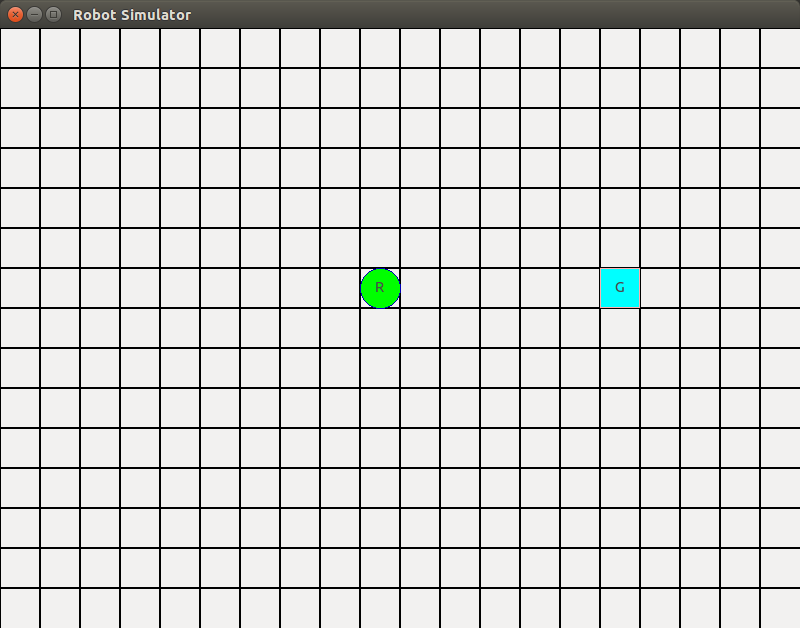
\includegraphics[trim = 80mm 80mm 20mm 70mm, clip, width = 2.4in, height = 1.6in]{robot_sim.png}
\end{figure}
We define the fitness of a potential solution to be:
$$fitness = \frac{2^{goalReached}}{1.0 + finalDistanceFromGoal + actionsTaken}$$

\subsection{Experimental Set Up}

\subsection{Results}


  \begin{figure}
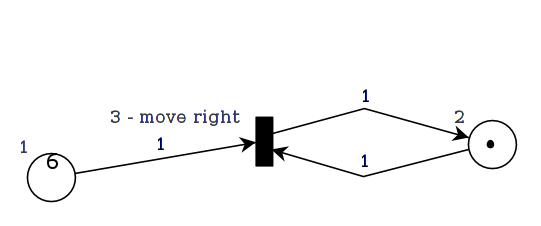
\includegraphics[scale=0.3]{PetriNet_1_1}

\end{figure}
\vspace{-5ex}
\begin{figure}
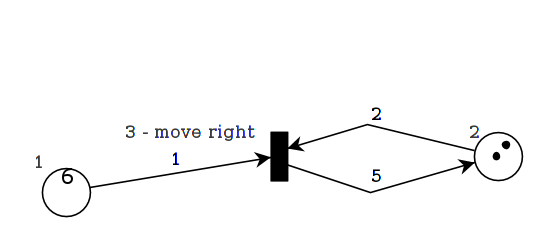
\includegraphics[scale=0.3,width=2in]{PetriNet_1_2}

\end{figure}
  \begin{figure}
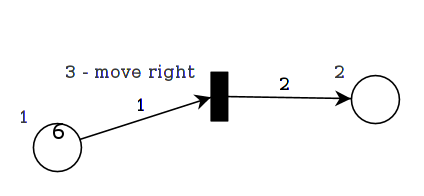
\includegraphics[scale=0.3]{PetriNet_1_3}
\vspace{-5ex}
\end{figure}
 \begin{figure}
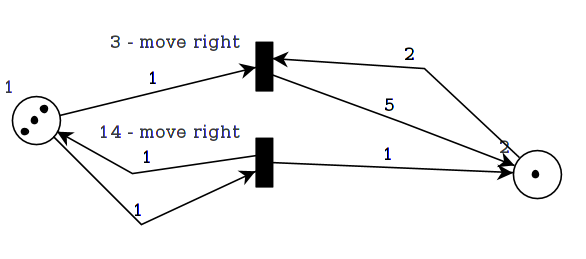
\includegraphics[scale=0.3, width=2in]{PetriNet_1_4}

\end{figure}

\begin{figure}
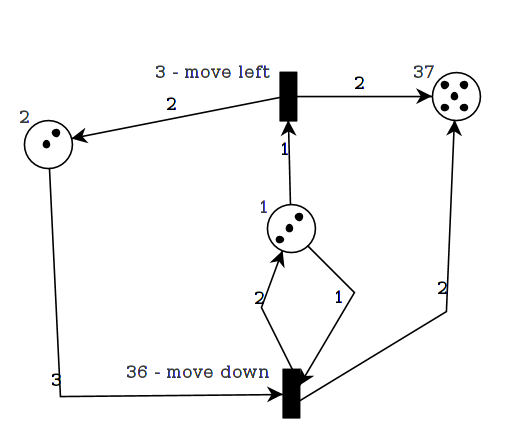
\includegraphics[scale=0.3]{PetriNet_2_1}
\end{figure}

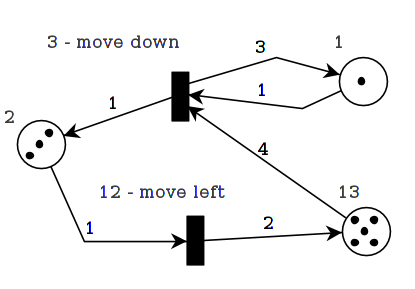
\includegraphics[scale=0.3]{PetriNet_2_2}

\section{Discussion and Future Work}

Conclusion: It is possible to evolve Petri nets
\begin{itemize}
\item Petri net weights, markings, and structure can adapt to improve network fitness.
\item Networks evolved through mutation can solve a given task.
\item Simple building blocks can create compound actions.
\end{itemize}

The next steps in exploring Petri net evolution are:
\begin{enumerate}
\item Add cross over operations to the evolutionary algorithm.
\item Explore different mutation operators.
\item Generate more complex types of Petri networks.
\item Increase the complexity of our target task.
\item Add methods to combine Petri nets into hierarchies.
\item Use reachability graph to simplify network.
\end{enumerate}

\section{Conclusion}

\bibliographystyle{plain}
\bibliography{project}

\end{document}